%%%%%%%%%%%%%%%%%%%%%%%%%%%%%%%%%%%%%%%%%%%%%%%%%%%%%%%%%%%%%%%%%%%%%%%%%%%%%%%%%%
\begin{frame}[fragile]\frametitle{Phase II}

Fine-tuning based approach:

\begin{itemize}
\item One limitation of 2D geometry-shape, represented as a sequential list of points, is that we can not represent line intersections or concentric loops. 
\item To address this a more comprehensive structure has been proposed which is based on the corresponding 3D structure popular in Solid Modeling, called Brep (Boundary Representation).
\end{itemize}	

\end{frame}


%%%%%%%%%%%%%%%%%%%%%%%%%%%%%%%%%%%%%%%%%%%%%%%%%%%%%%%%%%%%%%%%%%%%%%%%%%%%%%%%%%
\begin{frame}[fragile]\frametitle{Idea}

Leverage a geometry representation similar to that found in 3D B-rep (Boundary representation), but in 2D. It can be shown as:

\begin{lstlisting}
{
 'ShapeName': 'I',
 'Profile': [(5.0, 5.0), (10.0, 5.0), (10.0, 20.0), (5.0, 20.0)],
 'Midcurve': [(7.5, 5.0), (7.5, 20.0)],
 'Profile_brep': {
    'Points': [(5.0, 5.0), (10.0, 5.0), (10.0, 20.0),(5.0, 20.0)], # list of (x,y) coordinates
    'Lines': [[0, 1], [1, 2], [2, 3], [3, 0]], # list of point ids (ie index in the Points list)
                'Segments': [[0, 1, 2, 3]] # list of line ids (ie index in Lines list)
    },
 'Midcurve_brep': {
    'Points': [(7.5, 5.0), (7.5, 20.0)],
    'Lines': [[0, 1]],
                'Segments': [[0]]
    },    
}
\end{lstlisting}	
\end{frame}

%%%%%%%%%%%%%%%%%%%%%%%%%%%%%%%%%%%%%%%%%%%%%%%%%%%%%%%%%%%%%%%%%%%%%%%%%%%%%%%%%%
\begin{frame}[fragile]\frametitle{Data}

         \begin{center}
	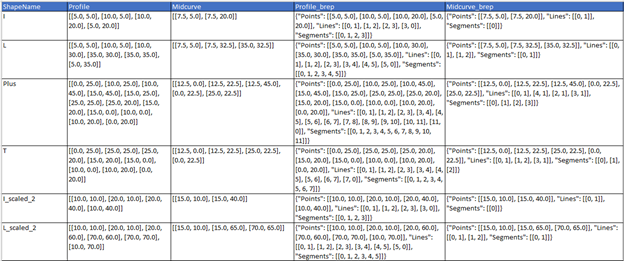
\includegraphics[width=\linewidth]{images/shapes_csv}
	\label{fig_csv}
    \end{center}
	
\end{frame}

%%%%%%%%%%%%%%%%%%%%%%%%%%%%%%%%%%%%%%%%%%%%%%%%%%%%%%%%%%%%%%%%%%%%%%%%%%%%%%%%%%
\begin{frame}[fragile]\frametitle{Data Explanation}

Column information is as below:

\begin{itemize}
\item ShapeName (text): name of the shape. Just for visualization/reports.
\item Profile (text): List of Points coordinates (x,y) representing outer profile shape, typically closed.
\item Midcurve (text): List of Points coordinates (x,y) representing inner midcurve shape, typically open.
\item Profile\_brep (text): Dictionary in Brep format representing outer profile shape, typically closed.
\item Midcurve\_brep (text): Dictionary in Brep format representing inner midcurve shape, typically open.
\end{itemize}	

Each Segment is a continuous list of lines. In case of, say `Midcurve-T`, as there is an intersection, we can treat each line in a separate segment. In the case of 'Profile O', there will be two segments, one for outer lines and another for inner lines. Each line is a list of points, for now, linear. Points is a list of coordinates (x,y), later can be (x,y,z).

\end{frame}

%%%%%%%%%%%%%%%%%%%%%%%%%%%%%%%%%%%%%%%%%%%%%%%%%%%%%%%%%%%%%%%%%%%%%%%%%%%%%%%%%%
\begin{frame}[fragile]\frametitle{Data Resolution}

\begin{itemize}
\item Once we have this Brep representations of both, profile and the corresponding midcurve, in the text form, then we can try various machine translation approaches or LLM based fine tuning or few-shots prompt engineering.
\item One major advantage of text based method over image based method is that image output still has stray pixels, cleaning which will be a complex task. But the text method has exact points. It may just give odd lines, which can be removed easily.
\end{itemize}	


\end{frame}

%%%%%%%%%%%%%%%%%%%%%%%%%%%%%%%%%%%%%%%%%%%%%%%%%%%%%%%%%%%%%%%%%%%%%%%%%%%%%%%%%%
\begin{frame}[fragile]\frametitle{Data Viz}

\begin{lstlisting}[basicstyle=\tiny, breaklines=true, breakatwhitespace=true,label=lst:python]
from datasets import load_dataset, Dataset, DatasetDict

base_url = "/content/drive/MyDrive/ImpDocs/Work/AICoach/Notebooks/data/"
dataset = load_dataset("csv", data_files={"train": base_url + "midcurve_llm_train.csv",
                                          "test": base_url + "midcurve_llm_test.csv",
                                          "validation": base_url + "midcurve_llm_val.csv"})
DatasetDict({
    train: Dataset({
        features: ['ShapeName', 'Profile', 'Midcurve', 'Profile_brep', 'Midcurve_brep'],
        num_rows: 793
    })
    test: Dataset({
        features: ['ShapeName', 'Profile', 'Midcurve', 'Profile_brep', 'Midcurve_brep'],
        num_rows: 99
    })
    validation: Dataset({
        features: ['ShapeName', 'Profile', 'Midcurve', 'Profile_brep', 'Midcurve_brep'],
        num_rows: 100
    })
})

\end{lstlisting}

\end{frame}

%%%%%%%%%%%%%%%%%%%%%%%%%%%%%%%%%%%%%%%%%%%%%%%%%%%%%%%%%%%%%%%%%%%%%%%%%%%%%%%%%%
\begin{frame}[fragile]\frametitle{Data Preprocessing}

The dataset is used to fine-tune the base model called ``Salesforce/codet5-small''. Trained model is saved and used for inference on test samples.

\begin{lstlisting}[basicstyle=\tiny, breaklines=true, breakatwhitespace=true,label=lst:python]
from transformers import T5ForConditionalGeneration, AdamW, get_linear_schedule_with_warmup
import pytorch_lightning as pl

class CodeT5(pl.LightningModule):
    def __init__(self, lr=5e-5, num_train_epochs=15, warmup_steps=1000):
        super().__init__()
        self.model_name = "Salesforce/codet5-small"
        self.model = T5ForConditionalGeneration.from_pretrained(self.model_name)
        self.save_hyperparameters()
        
    def forward(self, input_ids, attention_mask, labels=None):
        outputs = self.model(input_ids=input_ids, attention_mask=attention_mask, labels=labels)
        return outputs        
        :
        :

model = CodeT5()

trainer = Trainer(max_epochs=5,accelerator="auto",# gpus=1,
                  default_root_dir="/content/drive/MyDrive/CodeT5/Notebooks/Checkpoints",
                  logger=wandb_logger,
                  callbacks=[early_stop_callback, lr_monitor])
trainer.fit(model)
\end{lstlisting}

\end{frame}

%%%%%%%%%%%%%%%%%%%%%%%%%%%%%%%%%%%%%%%%%%%%%%%%%%%%%%%%%%%%%%%%%%%%%%%%%%%%%%%%%%
\begin{frame}[fragile]\frametitle{Inferencing}

The output predicted far away from the corresponding ground truth. 

There could be many reasons for the mismatch such as the quality of LLM, training parameters, and above all, need for a far bigger dataset for fine-tuning. But overall, the approach and preliminary results look promising to warrant further investigations.

\begin{lstlisting}[basicstyle=\tiny, breaklines=true, breakatwhitespace=true,label=lst:python]
input_ids = tokenizer(test_example['Profile_brep'], return_tensors='pt').input_ids
outputs = model.generate(input_ids)

print("Ground truth:", test_example['Midcurve_brep'])
print("Generated Midcurve:", tokenizer.decode(outputs[0], skip_special_tokens=True))

Ground truth: "{\"Points\": [[-8.4, 3.28], [-20.68, -5.33]], \"Lines\": [[0, 1]], \"Segments\": [[0]]}"
Generated Midcurve: "{\"Points\": [[-8.83, 4.32], [-21.23
\end{lstlisting}

\end{frame}